\section{一些基本知识}

\begin{quotation}
“量子力学在物理理论中占有一个很不平常的地位;它把经典力学作为一种极限情形而包含之,但在它的自身表述中,同时又需要这一极限情形。”\qquad 朗道
\end{quotation}

\subsection{频率,波长和波数}

根据量子力学,原子的状态可用一系列分立的能级表示。能级间可能发生跃迁,同时发出或吸收一个光子。假设跃迁发生在较低能级$i$,和较高能级$j$之间,则光子所携带的能量满足:

\begin{equation}\label{Planck Relation}
    \Delta E = E_j - E_i = h \nu = \frac{hc}{\lambda} = hc \sigma,
\end{equation}

这里$\nu$是光的频率\index{Frequency: 频率},$c$是光速\index{Speed of light: 光速},$h=6.626068 \times 10^{-34} J\cdot
s$是普朗克常数,$h
\nu$是一个光子携带的能量,$\lambda$是光在真空中的波长\index{Wavelength: 波长},$\sigma =
\frac{1}{\lambda}$是光在真空中的波数(wavenumber)\index{Wavenumber: 波数}。

一个跃迁就对应于光谱中的一条谱线,谱线的位置可用能量,频率,波长或波数来表示。能量常用的单位是$eV$,频率常用的单位是赫兹($Hz$),波长的常用单位是纳米($nm$),埃($0.1nm$),微米($\mu m ,
10^{-6}m$)。波数的常用单位是$cm^{-1}$。


\begin{center}

\begin{tabular}{|l|}
  \hline
  % after \\: \hline or \cline{col1-col2} \cline{col3-col4} ...

例:$1eV$的光,对应的频率($Hz$),波长($nm$)和波数($cm^{-1}$)\\各是多少?\\

  \hline
\end{tabular}

\end{center}

解: 电子电量: $e = 1.602 \times 10^{-19}C$, $1eV = 1.602 \times
10^{-19} J$

考虑, 光子能量: $\varepsilon = h \nu$, 普朗克常数: $h=6.626 \times
10^{-34} J \cdot s$,

\begin{equation*}
\nu = \frac{1.602 \times 10^{-19} J}{6.626 \times 10^{-34} J \cdot
s}= 2.4 \times 10^{14} Hz
\end{equation*}

利用: $c=\lambda \nu$, $\lambda = c / \nu$,

\begin{equation*}
\lambda = \frac{3.0 \times 10^8 m \cdot s^{-1}}{2.4 \times 10^{14}
Hz}=1.25 \times 10^{-6}m = 1250 nm
\end{equation*}

波数($\lambda^{-1}$)是,

\begin{equation*}
\frac{1}{\lambda} = \frac{1}{1.25 \times 10^{-6}m}=8.0\times 10^5
m^{-1}=8000 cm^{-1}
\end{equation*}

对HCl的分子的``振动-转动''光谱而言, 存在波数为$20.68 cm^{-1}$的谱线,
对应的能量是: $\thicksim 0.0026 eV$ 或 $\thicksim 6.0 \times
10^{11}Hz = 0.6 \text{THz}$.


\subsection{吸收,辐射和自发辐射}

假设原子中存在较低能态$i$,和较高能态$j$,处在$i$态的原子吸收$h\nu_{ji}=E_j
- E_i$的光可跃迁到$j$态。天文学中需要经常研究吸收谱(absorption
spectra),比如远处恒星发出的光(可看作是黑体辐射)穿过具有浓厚大气行星的大气层时,
就会发生吸收,根据吸收谱我们可推断太阳系外行星(exoplanet)的大气组分。



吸收谱的强度(或明暗对比度)正比于跃迁速率($B_{ij}\rho(\nu)$,
这里$B_{ij}$是吸收系数,
$\rho(\nu)$是电磁辐射场的能量密度),正比于处在$i$态的原子数$N_i$,
也正比于吸收光子的能量($h \nu_{ji}$),可表示为:


\begin{equation}\label{Absorption}
    N_i h \nu_{ji} B_{ij} \rho(\nu)
\end{equation}


辐射($j \to i$),可分为自发辐射(spontaneous
emission)\index{Spontaneous
emission: 自发辐射}和受激辐射(stimulated
emission)\index{Stimulated emission: 受激辐射}两个过程。“受激”意味着存在外加电磁辐射场,原子和电磁辐射发生相互作用。我们一般对电磁辐射做准经典的处理,即电磁辐射足够强,相当于有很多个光子,不需要引入对电磁辐射的量子化(即场量子化)。

如果只考虑吸收,和受激辐射两个过程,原子(处在$j$态)的状态数无法达到平衡,
此时必须考虑处在$j$态的原子会自发地向$i$态跃迁并发出一个光子的过程,
才能使$\frac{dN_j}{dt} = 0$。由于这个过程只涉及一个光子,
原则上必须引入对电磁辐射的量子化。

爱因斯坦通过考虑统计平衡条件得到了自发辐射系数$A_{ji}$,我们用下式表示发射谱的强度:

\begin{equation}\label{Emission}
    N_j h \nu_{ji} A_{ji},
\end{equation}

这里$N_j$是处在较高能级$j$原子的个数。我们也称$A_{ji}$是爱因斯坦$A$系数,而$B_{ij}$为爱因斯坦$B$系数。
爱因斯坦证明\footnote{参考: Einstein, ``Quantum theory of
radiation'' (1917)

\index{Einstein coefficients: 爱因斯坦系数}

\url{http://web.ihep.su/dbserv/compas/src/einstein17/eng.pdf}},它们满足:

\begin{equation}\label{AB coefficients}
    B_{ij}= \frac{c^3}{8 \pi h \nu_{ji}^3} \frac{g_j}{g_i} A_{ji},
\end{equation}

这里的$g_i$和$g_j$分别是态$i$和$j$的简并度。

我们一般用爱因斯坦$A$系数来表述跃迁发生的强度,单位为$s^{-1}$,
用其倒数($A^{-1}$)来表示跃迁发生的时间尺度(也可理解为原子处在$j$态的寿命),单位为$s$。


\subsection{爱因斯坦辐射理论}

首先回忆黑体辐射相关知识, 黑体辐射能量密度$u_T(\nu)$是:

\begin{equation*}
u_T (\nu ) = \frac{{8\pi h\nu ^3 }}{{c^3 }} \cdot
\frac{1}{{e^{\frac{{h\nu }}{{k T}}}  - 1}}
\end{equation*}

这就是所谓普朗克分布律(Planck law), 对低温$T \to 0$, $e^{h\nu/kT} -
1 \approx e^{h\nu/kT}$, 得到维恩分布律(Wien law):

\begin{equation*}
u_T(\nu)=\frac{8 \pi h \nu^3}{c^3} e^{-h\nu/kT}.
\end{equation*}


对高温$T \to \infty$, $e^{h\nu/kT} \approx 1 + \frac{h\nu}{kT}$,
普朗克分布律会退化为``瑞利-金斯分布律''(Rayleigh–Jeans law):

\begin{eqnarray*}
% \nonumber to remove numbering (before each equation)
  u_T(\nu) &=& \frac{8\pi h \nu^3}{c^3} \frac{kT}{h\nu} \\
  {} &=& \frac{8\pi \nu^2}{c^3}kT
\end{eqnarray*}

\begin{figure}[h]
\begin{center}
  % Requires \usepackage{graphicx}
  \includegraphics[width=5cm]{Spectrum/einstein-ab.ps}\\
  \caption{原子的``自发辐射'',``受激辐射''和``吸收''过程.}\label{Einstein AB coefficients}
\end{center}
\end{figure}


现在考虑N个原子与热辐射场$u_T(\nu)$间的相互作用,
原子中存在着两个能级, 一个是基态$i$, 一个是激发态$j$,
原子和热辐射场达到了热平衡, 平衡温度是$T$.

假设处在激发态的原子数为$N_j$,
并且假设基态简并度$g_i$和激发态简并度$g_j$都是1, 即$g_i = g_j =1$.

存在以下三种机制可使$N_j$发生变化,

(1)自发辐射过程($j \to i$), 使$N_j$减少:

\begin{equation*}
   \left( \frac{dN_j}{dt}\right)_1 = - A_{ji}N_j
\end{equation*}

即$N_j$的减少正比于自发辐射系数$A_{ji}$,
也正比于处在$j$态原子的数目$N_j$。
由上式也可计算出原子处在``激发态的平均寿命''\footnote{参考:杨福家《原子物理学》,
pp136.}是:

\begin{equation}\label{life time for excited states}
    \tau = \frac{1}{A_{ji}}
\end{equation}


(2)受激辐射($j \to i$), 使$N_j$减少:

\begin{equation*}
\left( \frac{dN_j}{dt} \right)_2 = - B_{ji}N_j \rho(\nu)
\end{equation*}

即$N_j$的减少正比于B系数($B_{ji}$), 处在$j$态的原子数目$N_j$,
也正比于电磁辐射场的能量密度$\rho(\nu)$.

(3)吸收过程($i \to j$), 使$N_i$增加:

\begin{equation*}
\left( \frac{dN_j}{dt} \right)_3 = B_{ij}N_i \rho(\nu)
\end{equation*}

即$N_j$的增加正比于B系数$B_{ij}$, 处在$i$态的原子数目$N_i$,
也正比于电磁辐射场的能量密度$\rho(\nu)$.

平衡条件:$\frac{dN_j}{dt}=\left( \frac{dN_j}{dt} \right)_1 + \left(
\frac{dN_j}{dt} \right)_2 + \left( \frac{dN_j}{dt} \right)_3 = 0$,
即:

\begin{equation}\label{equilibrium condition for AB}
B_{ij}N_i \rho(\nu) = B_{ji}N_j \rho(\nu) + A_{ji}N_j
\end{equation}

假设: $B_{ij}=B_{ji}$, 这是个很直观的假设, 平衡态下$i \to
j$的几率与$j \to i$的几率相等, 否则就不会平衡,
这就是所谓``细致平衡''(Detailed balancing).

\index{Detailed balancing: 细致平衡}

解出:

\begin{equation*}
\rho(\nu) = \frac{A_{ji}N_j}{B_{ij}N_i -
B_{ji}N_j}=\frac{A_{ji}}{B_{ji}}\frac{1}{\frac{N_i}{N_j}-1}
\end{equation*}

由于N个原子本身也处在热平衡态下, 根据玻尔兹曼分布律: $N_i \propto
e^{-E_i/kT}$, $N_j \propto e^{-E_j/kT}$, $\frac{N_i}{N_j} =
e^{(E_j-E_i)/kT}=e^{h\nu_{ji}/kT}$. 即:

\begin{equation*}
\rho(\nu) =\frac{A_{ji}}{B_{ji}}\frac{1}{e^{h\nu_{ji}/kT}-1}
\end{equation*}

回忆普朗克公式: $u_T (\nu ) = \frac{{8\pi h\nu ^3 }}{{c^3 }} \cdot
\frac{1}{{e^{\frac{{h\nu }}{{k T}}}  - 1}}$, 得到:

\begin{equation*}
\frac{A_{ji}}{B_{ji}}=\frac{{8\pi h\nu_{ji} ^3 }}{{c^3 }}
\end{equation*}

这说明自发辐射的选择定则与受激辐射和吸收的选择定则相同。


\subsection*{细致平衡条件}

在以上推导中, 我们假设了``细致平衡'': $B_{ij}=B_{ji}$, 如果考虑$g_j
\ne 1$, $g_i \ne 1$, 这个条件会变得不那么``直观''和``显然''.



由公式(\ref{equilibrium condition for AB}),

\begin{equation*}
\rho(\nu)=\frac{A_{ji}N_j}{B_{ij}N_i -
B_{ji}N_j}=\frac{A_{ji}}{B_{ij}\frac{N_i}{N_j}-B_{ji}}=\frac{A_{ji}}{B_{ij}\frac{g_i}{g_j}e^{h\nu_{ji}/kT}-B_{ji}}
\end{equation*}

继续化简可得:

\begin{equation*}
\rho(\nu)=\frac{A_{ji}g_j}{B_{ij}g_ie^{h\nu_{ji}/kT}-B_{ji}g_j}
\end{equation*}


\index{Detailed balancing: 细致平衡}

\begin{figure}[h]
\begin{center}
  % Requires \usepackage{graphicx}
  \includegraphics[width=6cm]{Spectrum/detailed_balancing_gij.ps}\\
  \caption{细致平衡: $j$态跃迁到$i$态}\label{detailed balancing graph}
\end{center}
\end{figure}

为了得到$u_T(\nu)$,
必须假设细致平衡\footnote{参考:褚圣麟《原子物理学》, pp68;

和``J J Sakurai, Modern Quantum Mechanics, pp334'', 现简述思路如下,

假设$i$态, 简并度为$g_i$; $j$态, 简并度为$g_j$.

粒子处在$i$态, 跃迁到$j$态的概率是: $w_{ij} \propto B_{ij} \propto
\left\langle V_{ij} \right\rangle^2 g_j$;

粒子处在$j$态, 跃迁到$i$态的概率是: $w_{ji} \propto B_{ji} \propto
\left\langle V_{ji} \right\rangle^2 g_i$.

由于: $\left\langle V_{ij}\right\rangle^2 = \left\langle
V_{ji}\right\rangle^2$,
即每个量子态跃迁到每个量子态的``可逆微观过程''几率相等,
见图(\ref{detailed balancing graph}). 所以:

\begin{equation*}
\frac{B_{ij}}{g_j} = \frac{B_{ji}}{g_i}
\end{equation*}

由上式可得到``细致平衡''条件:

\begin{equation*}
B_{ij}g_i = B_{ji}g_j
\end{equation*}}: $B_{ij}g_i = B_{ji}g_j$, 然后得到:

\begin{equation*}
\rho(\nu)=\frac{A_{ji}g_j}{B_{ji}g_j
(e^{h\nu_{ji}/kT}-1)}=\frac{A_{ji}}{B_{ji}}\frac{1}{e^{h\nu_{ji}/kT}-1}
\end{equation*}

即:

\begin{equation*}
\frac{A_{ji}}{B_{ji}}=\frac{{8\pi h\nu_{ji} ^3 }}{{c^3 }}
\end{equation*}

对上式``分子''和``分母''同时乘以$g_j$,

\begin{equation*}
\frac{A_{ji}g_j}{B_{ji}g_j} =
\frac{A_{ji}g_j}{B_{ij}g_i}=\frac{{8\pi h\nu_{ji} ^3 }}{{c^3 }}
\end{equation*}


因此: $B_{ij}= \frac{c^3}{8 \pi h \nu_{ji}^3} \frac{g_j}{g_i}
A_{ji}$, 即公式(\ref{AB coefficients}).

\subsection{氢原子光谱}

\subsubsection{四个量子数}

氢原子的哈密顿量可写为:

\begin{equation}\label{Hydrogen atom}
    H=-\frac{\hbar^2}{2 \mu} \nabla^2 - \frac{e^2}{4\pi\epsilon_0 r},
\end{equation}

即单个电子($-e$)库伦势场中的运动。在球坐标系($r,\theta,\phi$)下,求解薛定谔方程$H
\psi = E \psi$,得到本征波函数:

\begin{equation}\label{Wave Function for H atom}
    \psi(r, \theta, \phi) = R_{nl}(r) Y_{lm}(\theta,\phi)
\end{equation}

考虑到电子有自旋,$s=1/2, s_z= \pm
1/2$,单电子的运动状态(即原子的状态)可用$n$, $l$, $m$,
$s_z$四个量子数来表示。

$n$:主量子数,$n=1,2,3,...$,$n-1$对应节点数(严格说是$n-l-1$),即波函数通过原点的次数。对哈密顿(\ref{Hydrogen
atom})而言,氢原子的能量将只由$n$决定。

$l$:角量子数,$l =
0,1,2,...,n-1$,对单电子的轨道角动量,我们经常用小写字母$s, p, d, f,
g, ...$来表示$l = 0,1,2,...,n-1$。具体可见下表:


\begin{center}

\begin{tabular}{|c|c|c|c|c|c|c|c|c|c|}
  \hline
  % after \\: \hline or \cline{col1-col2} \cline{col3-col4} ...
  0 & 1 & 2 & 3 & 4 & 5 & 6 & 7 & 8 & ... \\
  s & p & d & f & g & h & i & k & l & ... \\
  \hline
\end{tabular}

\end{center}

$m$:磁量子数,对特定$l$,$m = 0,\pm 1, \pm 2,...\pm
l$,共$2l+1$种取值的可能性。

$s_z$:电子自旋在$z$轴方向上的投影,$s_z=\pm 1/2$。

总波函数可写成轨道部分$\psi_{nlm}(r,\theta,\phi)$乘以自旋部分$\chi(s_z)$的形式,
即:

\begin{equation*}
\Psi = \psi_{nlm}(r,\theta,\phi)\chi(s_z)
\end{equation*}


\subsubsection{跃迁的选择定则}

根据量子力学, 我们可以计算跃迁的选择定则. 对电偶极跃迁而言,
选择定则是:


\begin{eqnarray}
% \nonumber to remove numbering (before each equation)
  \Delta m &=& 0, \pm 1 \\
  \Delta l &=& \pm 1
\end{eqnarray}


这个选择定则对紫外线和可见光, 即波长远远大于原子半径适用.
对于波长与原子半径差不多的X射线, 则要考虑高级辐射, 比如四级辐射。

\subsubsection{相对论修正的氢原子}

玻尔模型(1913):

\begin{equation*}
T(n) = \frac{R}{n^2}
\end{equation*}


准量子力学的推导(索末菲, 1916):

\begin{equation*}
T(n,k)=\frac{R}{n^2}+\frac{R\alpha^2}{n^4}\left(
\frac{n}{k}-\frac{3}{4}\right)+...,
\end{equation*}

这里$k=1,2,...,n$.

未考虑自旋的量子力学推导(海森堡, 1926):

\begin{equation*}
T(n,l) = \frac{R}{n^2} + \frac{R\alpha^2}{n^4}\left(
\frac{n}{l+\frac{1}{2}}-\frac{3}{4} \right)
\end{equation*}

这里$l=0,1,2,...,n-1$.

\index{Fine-structure constant: 精细结构常数}

修正项能量对应就是精细结构(Fine structure),
相当于是0级结构的$\alpha^2$, 即小约4个数量级。


\subsection*{阅读}

Einstein, ``Quantum theory of radiation'' (1917)

\url{http://web.ihep.su/dbserv/compas/src/einstein17/eng.pdf}